\section{Maxwell-Boltzmann Verteilung}
Die Maxwell-Boltzmann Verteilung ist eine Funktion welche die 
Wahrscheinlichkeitsdichte beschreibt. Kurz um gibt
diese an, wie viele Teilchen in \% welche Geschwindigkeit haben 
für eine gegebene Temperatur. Wenn etwas wärmer wird, dann wird 
der Anteil schneller Teilchen zunehmen und der Anteil langsamer
Teilchen wird kleiner. Dieser Zusammenhang ist in der Abbildung
\ref{fig:dichte} dargestellt.

\begin{figure}[h!]
	\centering
	\begin{tikzpicture}[domain=0:4]
		\draw[->] (0,0) -- (4.5,0) node[below] 
			{$\vec{v}\,\left[\frac{m}{s}\right]$};
		\draw[->] (0,0) -- (0,2.5) node[left] 
			{$p(\vec{v})\,\left[\frac{s}{m}\right]$};

		\draw[color=red, samples=200, thick] plot[id=l] 
			function{1*(x*x)*exp(-0.5*x*x)};
		\draw[color=green, samples=200, thick] plot[id=m] 
			function{3*(x*x)*exp(-1*x*x)};
		\draw[color=blue, samples=200, thick] plot[id=h] 
			function{10*(x*x)*exp(-2*x*x)};

		\draw[color=red] (3,2) node[right] {Heiss};
		\draw[color=green] (3,1.5) node[right] {Warm};
		\draw[color=blue] (3,1) node[right] {Kalt};
	\end{tikzpicture}
	\caption{Wahrscheinlichkeitsdichte}
	\label{fig:dichte}
\end{figure}
Diese Wahrscheinlichkeitsdichte ist parametriert durch die Molekülmasse
$m_{kül}$ und die Temperatur $T$.
\[ \boxed{f(v) 
	= 4 \pi \left(\frac{m_{kül}}{2 \pi \cdot k_B \cdot T}\right)
	^{\frac{3}{2}} \cdot v^2 \cdot e^{-\left(\frac{m_{kül} \cdot v^2}
	{2 \cdot k_B \cdot T}\right)}
} \]

Die Funktion kann aber auch mit der molaren Masse eingesetzt werden. 
\[ \boxed{f(v) 
	= 4 \pi \left(\frac{m_{mol}}{2 \pi \cdot R \cdot T}\right)
	^{\frac{3}{2}} \cdot v^2 \cdot e^{-\left(\frac{m_{mol} \cdot v^2}
	{2 \cdot R \cdot T}\right)}
} \]


Um die Wahrscheinlichkeit zu erhalten, dass Teilchen sich mit einer 
Geschwindigkeit zwischen $\vec{v}_1$ und $\vec{v2}$ bewegen, muss
die Dichtefunktion integriert werden über diesem Intervall.
Dies ist in der Abbildung \ref{fig:wahrscheinlichkeit} dargestellt.
Wichtig ist zu beachten, dass ein Intervall der Art 
$[\vec{v}_1,\infty]$ manche Taschenrechner überfordert. Für solche
Intervalle empfiehlt es sich, das Intervall zu kehren auf 
$[0, \vec{v}_1]$ und das Ergebnis von $1$ abzuziehen.
\[ \boxed{P(v_1, v_2) 
	= \int\limits_{\vec{v}_1}^{\vec{v}_2} f(v)\,dv
	= 1 - \int\limits_{\vec{v}_2}^{\vec{v}_1} f(v)\,dv
} \]

\begin{figure}[h!]
	\centering
	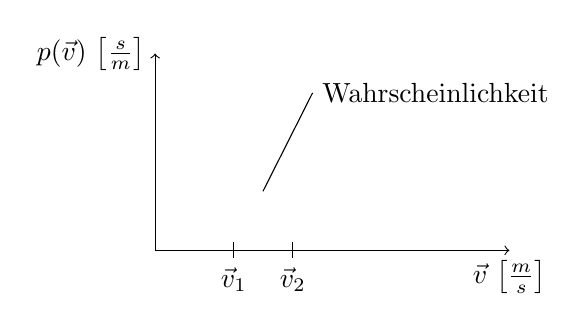
\begin{tikzpicture}[domain=0:4]
		\draw[->] (0,0) -- (4.5,0) node[below] 
			{$\vec{v}\,\left[\frac{m}{s}\right]$};
		\draw[->] (0,0) -- (0,2.5) node[left] 
			{$p(\vec{v})\,\left[\frac{s}{m}\right]$};

		\draw[color=blue, samples=200, thick] plot[id=h] 
			function{5*(x*x)*exp(-1*x*x)};

		\draw[fill=red!50, domain=1:1.75] plot[id=w] 
			function{5*(x*x)*exp(-1*x*x)} -- (1.75,0) -- (1,0) -- cycle;

		\draw[] (1,0.1) -- (1,-0.1) node[below] {$\vec{v}_1$};
		\draw[] (1.75,0.1) -- (1.75,-0.1) node[below] {$\vec{v}_2$};

		\draw[] (1.37,0.75) -- (2,2) node[right] {Wahrscheinlichkeit};
	\end{tikzpicture}
	\caption{Wahrscheinlichkeit für $P(\vec{v}_1, \vec{v}_2)$}
	\label{fig:wahrscheinlichkeit}
\end{figure}

\section{Charakteristische Geschwindigkeiten}
Wahrscheinlichste Geschwindigkeit
\[ \boxed{v_w = \sqrt{\frac{2 \cdot k_B \cdot T}{m_{kül}}} 
= \sqrt{\frac{2 \cdot R \cdot T}{m_{mol}}}} \]
Durchschnittsgeschwindigkeit
\[ \boxed{v_{av} = \langle v \rangle 
= \sqrt{\frac{8 \cdot k_B \cdot T}{\pi \cdot m_{kül}}} 
= \sqrt{\frac{8 \cdot R \cdot T}{\pi \cdot m_{mol}}}} \]
Root Mean Square Geschwindigkeit
\[ \boxed{v_{rms} = \sqrt{\langle v^2 \rangle} 
= \sqrt{\frac{3 \cdot k_B \cdot T}{m_{kül}}} 
= \sqrt{\frac{3 \cdot R \cdot T}{m_{mol}}}} \]
